\graphicspath{{./Chapters/CH4/Pictures/}}
\let\cleardoublepage\clearpage

\section{Overview}
\label{subsec:ch4-overview}

This chapter closes the gap between the ideal drive models used so far and the bench-realistic behavior observed on hardware. We proceed in two stages. First, we measure and identify the permanent-magnet synchronous motor (PMSM) parameters needed by analysis and control—stator resistance, synchronous inductances (or \(L_d,L_q\)), permanent-magnet flux linkage, pole pairs, and the mechanical pair \((J,B)\) with optional Coulomb friction. The emphasis is on practical, repeatable procedures that can be executed with readily available instrumentation (e.g., an RLC meter and the drive).

Second, we model the inverter’s non-ideal behavior and show how it alters the voltages actually seen by the machine. The focus is on effects that matter most in low-speed, high-precision operation: dead time, device conduction drops and on-state resistances, current-polarity–dependent commutation asymmetries, and (when relevant) sampling/actuation delays and DC-bus ripple. We derive a compact average model that injects these distortions as additive biases to the ideal \(\alpha\beta/dq\) voltages, and we outline a straightforward bench characterization (“DC test”) that captures load-dependent deviations in a small lookup table. The identified motor parameters and the calibrated inverter model are then plugged into the simulation environment used throughout the thesis, providing a consistent basis for evaluating and tuning the model-predictive and PI–FOC controllers under realistic conditions.



\section{Motor Parameters Measurement}
\label{subsec:ch4-MotorParameters}
\subsection{Motor Stator Resistance Measurement}
The stator resistance \(R_s\) was measured with a two-wire LCR meter in series-RL mode at a low test frequency (typically 100–300 Hz), with the rotor stationary. For a wye-connected machine, the meter reading was taken line-to-line with the third terminal open, using the \emph{exact same long phase leads and harness} as in the bench setup—by design, no OPEN/SHORT compensation or lead subtraction was applied so that the identified resistance reflects the total copper path seen by the drive. Denoting the raw meter reading by \(R_{LL}^{(\mathrm{meas})}\), the per-phase value used in the \(dq\) model is
\[
R_s \;=\; \tfrac{1}{2}\,R_{LL}^{(\mathrm{meas})} =\tfrac{1}{2}\times 2.57~\Omega=1.25~\Omega.
\]
This harness-inclusive \(R_s=1.25~\Omega\) is the value adopted in the simulations and controller design.

MEASUREMENT SETUP SHOT FROM THE LAB HAS TO BE INCLUDED HERE.

\subsection{Motor Stator Inductance Measurement}
\label{subsec:Ls-osc}

Inductances are identified by measuring the electrical time constant on the oscilloscope and then converting it to \(L\) using the known phase resistance. At standstill, align the rotor electrically at \(0^\circ\) (d–axis) and apply a small DC step along the d–axis; record the current step response \(i_d(t)\). Repeat at \(90^\circ\) (q–axis) to obtain \(i_q(t)\). With \(\omega_e\simeq 0\) each axis behaves as a first–order system with time constant \(\tau\) measured at 63\% of the steady state current, so the inductances follow directly from the current respone measurements as shown in Figure~\ref{fig:fcs-diagram}:
\begin{figure}[h]
	\centering
	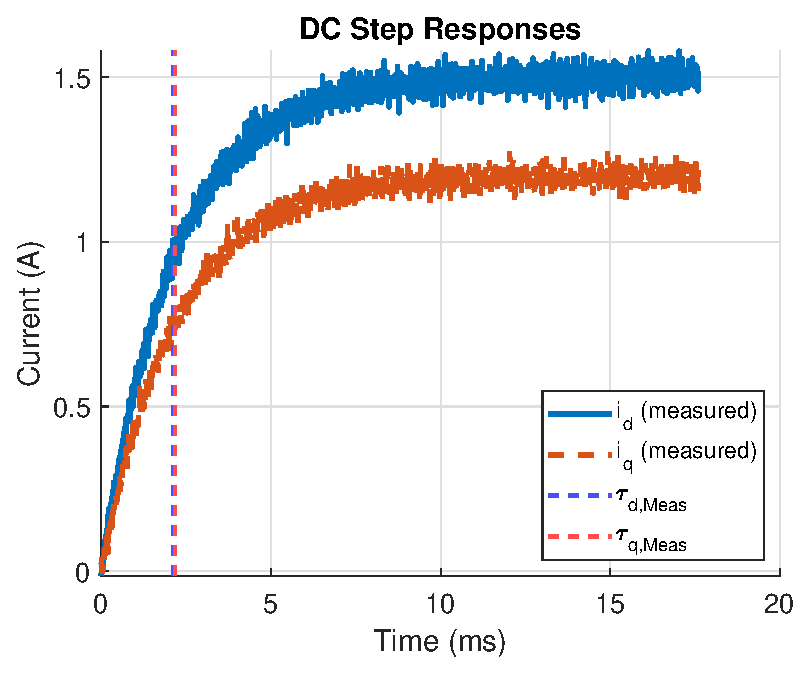
\includegraphics[width=\textwidth]{./InductanceMeas}
	\caption{DC-Step Test for Motor Inductance Measurements}
	\label{fig:InductanceMeas}
\end{figure}


With the previously identified per-phase resistance \(R_s=1.25~\Omega\), the motor inductances are then computed by the following equations:
\begin{equation}
\label{eq:Ld-from-tau-osc}
L_d \;=\; R_s\,\tau_d, 
\qquad
L_q \;=\; R_s\,\tau_q,
\end{equation}

Following the procedure above, \(\tau_d\) equals 2.1227~\text{ms}  and \(\tau_q\) equals 2.1716~\text{ms} were read from the oscilloscope, and the inductances were computed via \eqref{eq:Ld-from-tau-osc} with \(R_s=1.25~\Omega\), yielding
\[
L_d=2.67~\text{mH},\qquad L_q=2.75~\text{mH}.
\]
These are the inductance values used in the electrical model and subsequent controller design.

MEASUREMENT SETUP SHOT FROM THE LAB HAS TO BE INCLUDED HERE.

\subsection{Motor Flux Linkage Measurement}
\label{subsec:lambda-emf-ll}

The motor is driven as a generator by a prime mover at \(1000~\mathrm{rpm}\) with open stator terminals. Using a differential probe, the line–to–line no-load back-EMF is recorded on the oscilloscope as shown in Figure~\ref{fig:FluxLinkage} and its fundamental RMS value \(E_{\mathrm{LL,rms}}\) is extracted (single-tone FFT or narrowband filter at the electrical frequency). With pole–pair count \(p=4\), the speeds are
\[
\omega_m = 2\pi\frac{1000}{60}\ \text{rad/s},\qquad
\omega_e = p\,\omega_m,
\]
and the flux linkage is computed directly from the scope measurement by
\[
\lambda_f \;=\; \frac{\sqrt{2}}{\sqrt{3}}\;\frac{E_{\mathrm{LL,rms}}}{\omega_e}.
\]

Applying the above with the oscilloscope-measured \(E_{\mathrm{LL,rms}}\) at \(1000~\mathrm{rpm}\) gives
\[
\boxed{\lambda_f = 0.1227~\text{Wb}}.
\]

\begin{figure}[h]
	\centering
	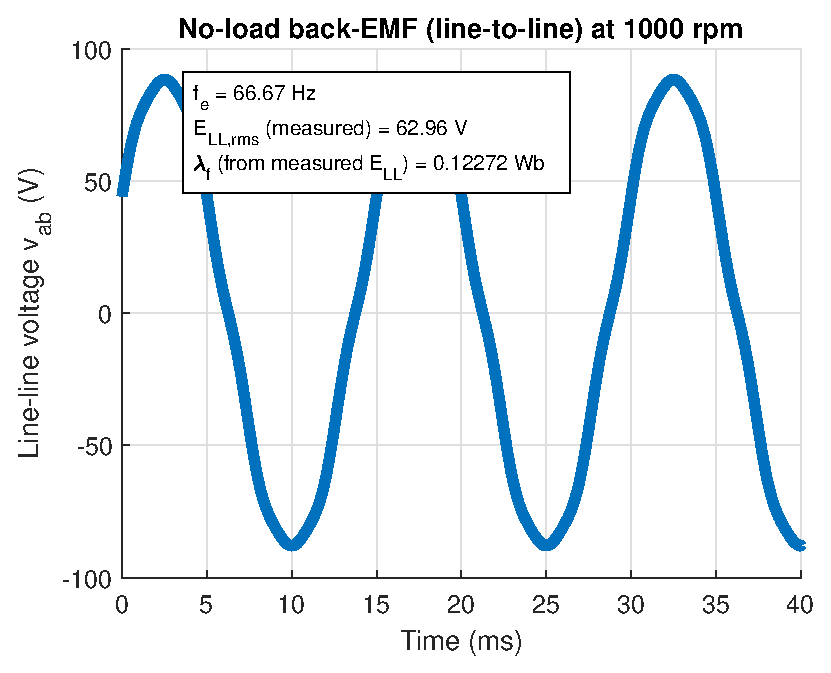
\includegraphics[width=\textwidth]{./FluxLinkageMeas}
	\caption{No-Load back-EMF Test at 1000 RPM}
	\label{fig:FluxLinkage}
\end{figure}


\subsection{Viscous Friction Measurement}
\label{subsec:viscous-friction}

The motor is driven at a sequence of constant mechanical speeds covering the operating range (e.g., from low rpm up to the rated region). At each target speed the drive is held until the signals stabilize—i.e., the speed derivative is negligible and the torque/current readings have settled—so that transients are removed. The steady values \((\omega_m,\,T_e)\) are then logged. Repeating this for all speed points produces a set of steady-state pairs suitable for identification.

A smooth curve of torque versus speed is drawn by interpolating the measured points to aid visualization. The friction parameters are obtained by fitting the standard affine model
\[
T_e(\omega_m)=B\,\omega_m+T_c,
\]
where the slope \(B\) is the viscous friction coefficient \([\mathrm{N\,m\,s/rad}]\) and the \emph{intercept} \(T_c\) is the constant (Coulomb) friction torque \([\mathrm{N\,m}]\). The line fit (ordinary least squares) is performed on the measured \((\omega_m,\,T_e)\) data as shown in Figure~\ref{fig:ViscousFriction}.

\begin{figure}[H]
	\centering
	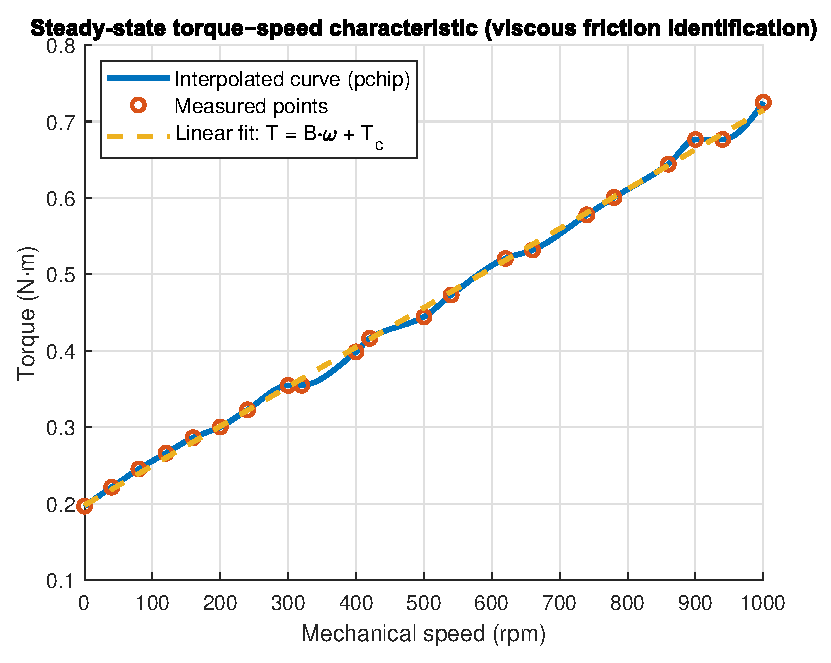
\includegraphics[width=\textwidth]{./ViscousFriction}
	\caption{Steady-State Torque-Speed Characteristic Test for Viscous Friction Identification}
	\label{fig:ViscousFriction}
\end{figure}

\subsection{Motor Inertia Measurement}
\label{subsec:inertia-coastdown}

The rotor inertia \(J\) is identified from a \emph{free deceleration} test. The motor is accelerated to a target speed and then commanded to zero electromagnetic torque (e.g., \(i_q\!\to\!0\) or inverter disabled). The mechanical speed \(\omega_m(t)\) is logged until near standstill. Under the viscous–Coulomb friction model used in this chapter,
\[
J\,\dot{\omega}_m \;=\; -\,B\,\omega_m \;-\; T_c,
\]
so a linear fit of \(\dot{\omega}_m\) versus \(\omega_m\) yields \(\dot{\omega}_m = a\,\omega_m + b\) with \(a=-B/J\) and \(b=-T_c/J\). 

Applying the above to the recorded coast–down data and using \(B=0.004775~\mathrm{N\,m\,s/rad}\) and \(T_c=0.2~\mathrm{N\,m}\), the identified rotor inertia is
\[
\boxed{J = 0.00636~\mathrm{kg\,m^2}}.
\]

\section{Inverter Non-Linearities Average Model for a Two-Level VSI}
\label{sec:vsi-nonlinear-model}

\subsection{Analytical Modeling}
In a PWM two-level voltage-source inverter (VSI) the actual pole voltages differ from the ideal SVM targets because of dead time, finite turn-on/off delays, and device on-state drops in the transistor and anti-parallel diode. The resulting mismatch introduces low-frequency distortion in the phase voltages, which propagates to current ripple, harmonic torque, and degraded tracking effects that are well documented in the literature. 

Consider one switching period \(T_s\). Let \(T_u^\ast,T_v^\ast,T_w^\ast\) be the ideal upper-device on-times produced by SVM. Practical gating inserts a dead interval so that each leg conducts slightly less (or slightly more) than scheduled depending on the current polarity. Defining \(\operatorname{sgn}(i_{ph})\!:=\!+1\) as shown in (\ref{eq:phasedir}) if the phase current flows into the machine and \(-1\) otherwise (sign convention as in Figure \ref{fig:InverterNonlinearities}), the average phase-to-neutral voltage including dead time \(t_{\mathrm{dead}}\), commutation skews \(t_{\mathrm{ON}},t_{\mathrm{OFF}}\), and device drops is given, per phase \(u\), by the standard form (\ref{eq:vun}), and (\ref{eq:vun_star}):

\begin{figure}[h]
	\centering
	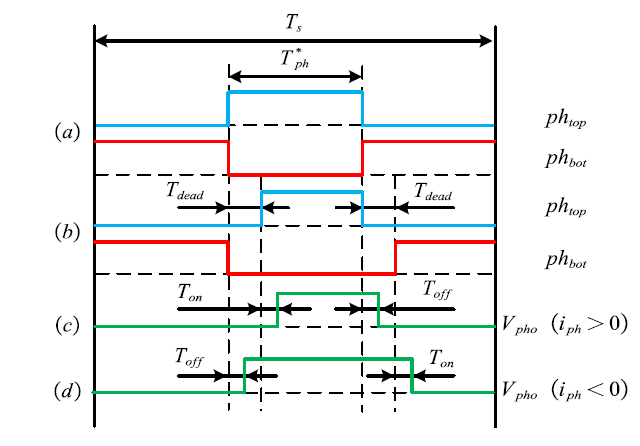
\includegraphics[width=\textwidth]{./InverterNonlinearities}
	\caption{Ideal versus non-ideal switching and the resulting phase voltage: (a) ideal gating waveforms; (b) gating with inserted dead time; (c) actual phase voltage for \(i_{ph}>0\); (d) actual phase voltage for \(i_{ph}<0\).}
	\label{fig:InverterNonlinearities}
\end{figure}


\begin{equation}
\label{eq:phasedir}
\operatorname{sgn}(i_{ph}) =
\begin{cases}
  1,  & i_{ph} > 0,\\[2pt]
 -1,  & i_{ph} < 0.
\end{cases}
\end{equation}

\begin{equation}
\label{eq:vun}
v_{un}=\frac{V_{\!dc}-V_{\!CE}+V_D}{3T_s}\,\bigl(2T_u-T_v-T_w\bigr)
-\frac{V_{CE0}+V_{D0}}{6}\bigl(2\,\operatorname{sgn}i_u-\operatorname{sgn}i_v-\operatorname{sgn}i_w\bigr)
-\frac{R_{CE}+R_D}{2}\,i_u,
\end{equation}
with the ideal counterpart
\begin{equation}
\label{eq:vun_star}
v_{un}^\ast=\frac{V_{\!dc}-V_{\!CE}+V_D}{3T_s}\,\bigl(2T_u^\ast-T_v^\ast-T_w^\ast\bigr).
\end{equation}
Here the transistor and diode drops are captured by the usual current\-dependent linearizations
\begin{equation}
\label{eq:lin-drops}
V_{\!CE}=V_{CE0}+R_{CE}\,\lvert i_{\!ph}\rvert,\qquad
V_D=V_{D0}+R_D\,\lvert i_{\!ph}\rvert,
\end{equation}
and the \emph{dead-time kernel}
\begin{equation}
\label{eq:Lambda}
\Lambda=\frac{(V_{\!dc}-V_{\!CE}+V_D)\,(t_{\mathrm{dead}}+t_{\mathrm{ON}}-t_{\mathrm{OFF}})}{3T_s}+\frac{V_{CE0}+V_{D0}}{6}
\end{equation}
collects the polarity-dependent bias. Equations \eqref{eq:vun}–\eqref{eq:Lambda} summarize the combined effect of dead time, timing skews, and device drops on the average phase voltage.

Stacking the three phases, the error \(\boldsymbol{v}_{\!err}=\boldsymbol{v}^\ast-\boldsymbol{v}\) admits a compact expression:
\begin{equation}
\label{eq:verr-abc}
\begin{bmatrix} v_{un}^{err}\\ v_{vn}^{err}\\ v_{wn}^{err}\end{bmatrix}
=\Lambda
\begin{bmatrix} 2&-1&-1\\ -1&2&-1\\ -1&-1&2\end{bmatrix}
\begin{bmatrix}\operatorname{sgn}i_u\\ \operatorname{sgn}i_v\\ \operatorname{sgn}i_w\end{bmatrix}
+\frac{R_{CE}+R_D}{2}\begin{bmatrix} i_u\\ i_v\\ i_w\end{bmatrix}.
\end{equation}
This makes two ingredients explicit: (i) a polarity kernel driven by current signs that flips as the phase currents cross zero, and (ii) a small resistive drop proportional to phase current.

Using the Clarke–Park transformations, the theoretical distortion voltages appearing in the synchronous model are
\begin{equation}
\label{eq:vdqth}
\begin{bmatrix} v_d^{th}\\ v_q^{th}\end{bmatrix}
= \;3\,K_{3s\!\to r}\,\Lambda
\begin{bmatrix}\operatorname{sgn}i_u\\ \operatorname{sgn}i_v\\ \operatorname{sgn}i_w\end{bmatrix}
+K_{3s\!\to r}\,\frac{R_{CE}+R_D}{2}\begin{bmatrix} i_u\\ i_v\\ i_w\end{bmatrix},
\end{equation}
where \(K_{3s\!\to r}\) is the standard \(3\! \to\! 2\) Park matrix evaluated at electrical angle \(\theta_e\),
\begin{equation}
\label{eq:K32}
K_{3s\!\to r}=\frac{2}{3}
\begin{pmatrix}
\cos\theta_e & \cos(\theta_e\!-\!2\pi/3) & \cos(\theta_e\!+\!2\pi/3)\\[2pt]
-\sin\theta_e & -\sin(\theta_e\!-\!2\pi/3) & -\sin(\theta_e\!+\!2\pi/3)
\end{pmatrix}\!.
\end{equation}
In this form the non\-idealities enter the \(dq\) electrical equations as an additive bias to the commanded voltages. The cited analysis further notes that bus voltage and dead time dominate the distortion magnitude; the impact weakens as operating speed rises, and the dominant ripple in \(dq\) appears around \(6\omega_e\) (six times the electrical frequency), consistent with three\-phase symmetry. 

With \(\boldsymbol{v}_{dq}^{th}\) known from \eqref{eq:vdqth}, the synchronous PMSM model reads
\begin{equation}
\label{eq:pmsm-with-dist}
\begin{bmatrix} v_d\\ v_q\end{bmatrix}
=\begin{bmatrix} R & -\omega_e L_q\\ \omega_e L_d & R\end{bmatrix}
\begin{bmatrix} i_d\\ i_q\end{bmatrix}
+\begin{bmatrix} 0\\ \omega_e\lambda_f\end{bmatrix}
+\begin{bmatrix} v_d^{th}\\ v_q^{th}\end{bmatrix},
\end{equation}
so that any controller (PI, MPC, or observer\-based) can treat \([v_d^{th}\ v_q^{th}]^\top\) as a known feedforward bias (``theoretical'' part) and reserve an estimator for the small residual coming from parameter spread or temperature.


\subsection{PI Controller Simulation Modeling Under Inverter-Nonlinearities Effects}
This section validates the complete drive model and controllers through a focused suite of studies: (i) steady-state operation to verify ripple, losses, and harmonic content; (ii) low-speed operation to probe back-EMF limits and non-idealities; (iii)  dynamic performance under speed/current steps; (iv) parameter variation to gauge robustness against model mismatch; and (v) load variation to assess torque disturbance rejection.
\subsubsection{Steady State Operation}
With dead time and device drops enabled, the PI drive at 1000 rpm exhibits high harmonic content that a moderate-bandwidth controller (\(\approx\)20~Hz) cannot suppress. At \emph{low load} (10\% rated torque, \(0.3~\mathrm{N\,m}\)) the phase-current THD reaches 16.4\% (see Fig.~\ref{fig:PINL_1000rpm_low}); at \emph{medium load} (50\% rated torque, \(1.75~\mathrm{N\,m}\)) it falls to 4.3\% (see Fig.~\ref{fig:PINL_1000rpm_med}). The pattern is consistent with PWM non-idealities injecting polarity-dependent voltage biases that map, via three-phase symmetry, into prominent \(5^\text{th}\) and \(7^\text{th}\) harmonics; because these behave as additive voltage sources rather than simple plant shifts, a PI loop with limited crossover cannot reject them effectively, yielding elevated THD even though average torque and speed regulation remain correct.

\begin{figure}[H]
  \centering
  % --- (a) Low load under non-ideal inverter ---
  \begin{subfigure}{0.485\textwidth}
    \centering
    % Replace with your exported plot/image
    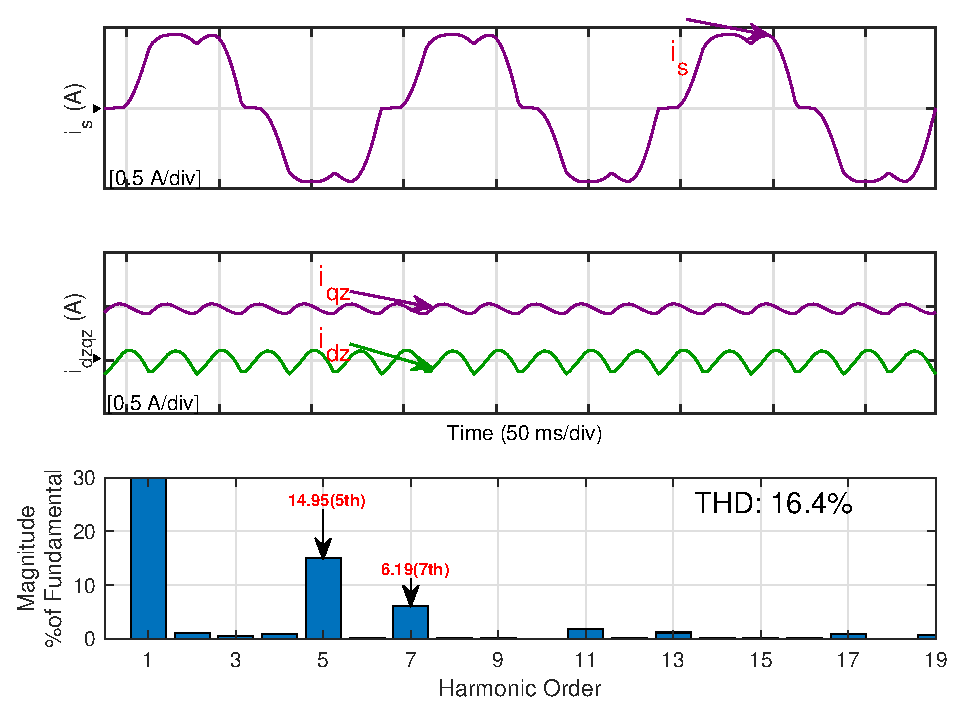
\includegraphics[width=\linewidth]{./PIMidSpeedLowLoadSteadyState}
    \caption{Low load: \(T=0.3~\mathrm{N\,m}\). \\THD \(=16.4\%\).}
    \label{fig:PINL_1000rpm_low}
  \end{subfigure}\hfill
  % --- (b) Medium load under non-ideal inverter ---
  \begin{subfigure}{0.485\textwidth}
    \centering
    % Replace with your exported plot/image
    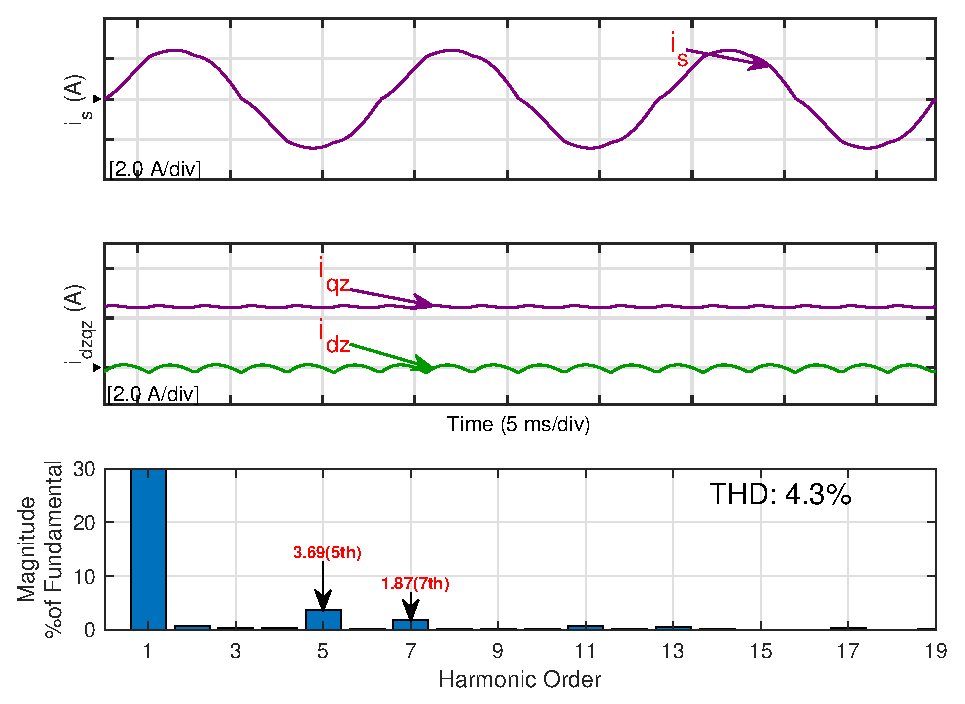
\includegraphics[width=\linewidth]{./PIMidSpeedMidLoadSteadyState}
    \caption{Medium load: \(T=1.75~\mathrm{N\,m}\).\\ THD \(=4.3\%\).}
    \label{fig:PINL_1000rpm_med}
  \end{subfigure}

  \caption{PI steady-state at 50\% rated speed (1000 rpm) with inverter non-linearities enabled (dead time, device drops). The figure reports  phase currents, \(d\)- and \(q\)-axis currents, and the THD.}
  \label{fig:PINL_1000rpm}
\end{figure}

\subsubsection{Low Speed Operation}
With dead time and device drops enabled, the PI drive at 200 rpm (10\% rated) shows pronounced distortion: at low load (10\% rated torque, \(0.3~\mathrm{N\,m}\)) the phase-current THD reaches 23.2\% (Fig.~\ref{fig:PINL_200rpm_low}), while at high load (100\% rated torque, \(3.5~\mathrm{N\,m}\)) it falls to 6.9\% (Fig.~\ref{fig:PINL_200rpm_high}). The pattern reflects polarity-dependent voltage biases that project into strong odd harmonics (notably \(5^\text{th}\)/\(7^\text{th}\)), which a PI loop with \(\approx\)20~Hz crossover cannot effectively reject. At 100 rpm (5\% rated), the same non-idealities consume much of the voltage headroom and the loop fails to settle—see Fig.~\ref{fig:PINL_100rpm_unstable}—indicating insufficient robustness of the present PI design in this extreme low-speed, non-ideal regime.

% Requires in preamble:
% \usepackage{graphicx}
% \usepackage{subcaption}

% ---------- PI @ 10% rated (200 rpm) under inverter non-linearities ----------
\begin{figure}[H]
  \centering
  % Low load (10% rated torque)
  \begin{subfigure}{0.485\textwidth}
    \centering
    % Replace with your exported plot/image
    
\includegraphics[width=\linewidth]{./PISteadyStateLowLoad200Rpm}
    \caption{Low load: \(T=0.3~\mathrm{N\,m}\). THD \(=23.2\%\).}
    \label{fig:PINL_200rpm_low}
  \end{subfigure}\hfill
  % High/rated load (100% rated torque)
  \begin{subfigure}{0.485\textwidth}
    \centering
    % Replace with your exported plot/image
    
\includegraphics[width=\linewidth]{./PISteadyStateHighLoad200Rpm}
    \caption{Rated load: \(T=3.5~\mathrm{N\,m}\). THD \(=6.9\%\).}
    \label{fig:PINL_200rpm_high}
  \end{subfigure}

  \caption{PI controller at 200 rpm (10\% rated) with inverter non-linearities enabled (dead time, device drops). Each panel shows The figure reports  phase currents, \(d\)- and \(q\)-axis currents, and the THD. Prominent odd harmonics (notably 5th/7th) elevate THD at low load; the higher fundamental at rated load reduces the relative distortion.}
  \label{fig:PINL_200rpm}
\end{figure}

% ---------- PI @ 5% rated (100 rpm) under inverter non-linearities: unstable case ----------
\begin{figure}[H]
  \centering
  % Replace with your exported plot/image
  
\includegraphics[width=0.6\linewidth]{./PISteadyStateLowLoad100Rpm}
  \caption{PI controller at 100 rpm (5\% rated) with inverter non-linearities enabled. The combination of dead time/device drops and limited loop bandwidth leads to failure to settle (unstable/oscillatory response). The figure reports  phase currents, \(d\)- and \(q\)-axis currents, and the THD.}
  \label{fig:PINL_100rpm_unstable}
\end{figure}

\subsubsection{Dynamic Performance}
With dead time and device drops enabled, speed steps within the 5–50\% band reveal a low-speed limitation: when the request includes 5\% (100~rpm), the PI loop fails to settle at both low load and rated load. For commands \(\mathbf{\ge}10\%\) of rated (200–1000~rpm), the same controller tracks cleanly with well-damped transients and negligible steady-state error. These behaviors are consolidated in the two summary plots: Fig.~\ref{fig:PINL_Dyn_low} (low load, multiple speed transitions) and Fig.~\ref{fig:PINL_Dyn_rated} (rated load, multiple speed transitions).

\begin{figure}[H]
  \centering
  % --- (a) Low load ---
  \begin{subfigure}{0.485\textwidth}
    \centering
    % Replace with your exported plot/image stacking multiple speed transitions
    
\includegraphics[width=\linewidth]{./DynamicResponsePILowLoad}
    \caption{Low load (\(T=0.3~\mathrm{N\,m}\)). Includes 5–50\% speed transitions; fails to settle at 5\% (100 rpm), tracks cleanly for \(\ge\)10\%.}
    \label{fig:PINL_Dyn_low}
  \end{subfigure}\hfill
  % --- (b) Rated load ---
  \begin{subfigure}{0.485\textwidth}
    \centering
    % Replace with your exported plot/image stacking multiple speed transitions
    
\includegraphics[width=\linewidth]{./DynamicResponsePIHighLoad}
    \caption{Rated load (\(T=3.5~\mathrm{N\,m}\)). Same behavior: unstable at 5\%, well-damped for \(\ge\)10\%.}
    \label{fig:PINL_Dyn_rated}
  \end{subfigure}

  \caption{PI dynamic performance under inverter non-linearities (dead time, device drops) with multiple speed transitions in the 5–50\% band. Each subfigure shows command vs.\ speed, \(i_q\), and phase currents. The controller fails to settle at 5\% (100 rpm) but tracks cleanly for \(\ge\)10\% of rated speed across both load conditions.}
  \label{fig:PINL_Dyn}
\end{figure}

\subsubsection{Parameter Variation}
To probe worst-case robustness, the PI controller was evaluated at 10\% rated speed (200~rpm) with inverter non-idealities (dead time, device drops) while the motor model used for tuning was biased by \(R_s{+}25\%\) and \(L_{d,q}{-}25\%\). This perturbation shortens the electrical time constant (\(\tau=L/R \rightarrow 0.60\,\tau\)), shifts the plant pole, and detunes the PI crossover/cutoff relative to the true plant. As illustrated in Fig.~\ref{fig:PINL_ParamVariation}, the phase-current THD increases from 23.2\% (nominal parameters) to 24.2\% under the bias—a modest but measurable degradation consistent with reduced disturbance-rejection margin when the PI bandwidth drifts in the presence of additive inverter distortion.
\begin{figure}[H]
  \centering
  % Replace with your exported composite plot (e.g., speed, dq-currents, phase currents, THD bars)
  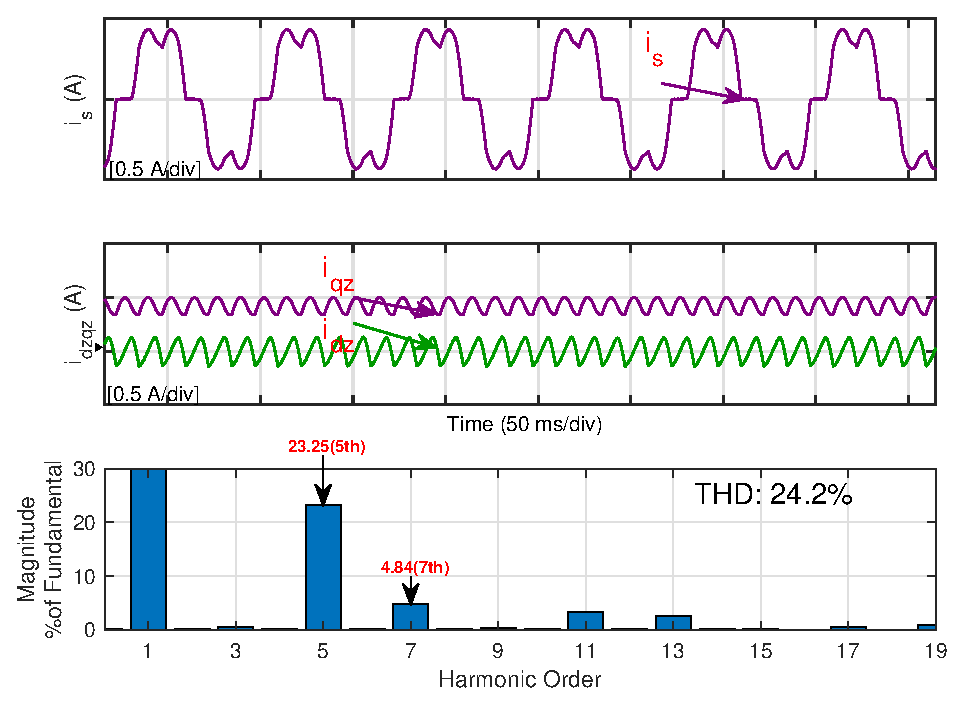
\includegraphics[width=0.8\linewidth]{./PIParameterVariation}
  \caption{PI controller under parameter variation with inverter non-linearities at 200 rpm (10\% rated).}
  \label{fig:PINL_ParamVariation}
\end{figure}

\subsubsection{Load Variation}	
With dead time and device drops enabled, the motor was held at 1000 rpm while the load torque was stepped from 10\% to 100\% of rated in 20\% increments, each plateau maintained to steady state. As shown in Fig.~\ref{fig:PINL_LoadVariation}, the PI loop preserves the commanded speed without appreciable droop; the \(q\)-axis current \(i_q\) rises in clean, proportional steps to furnish the added torque, and the phase currents—though exhibiting extra ripple from non-idealities—remain bounded and well behaved. Transients are short and well damped across all steps, evidencing robust disturbance rejection despite the inverter’s harmonic bias.
% Requires in preamble:
% \usepackage{graphicx}

\begin{figure}[H]
  \centering
  % Replace with your exported composite plot:
  % (left) speed response, (middle) q-axis current, (right) phase currents
  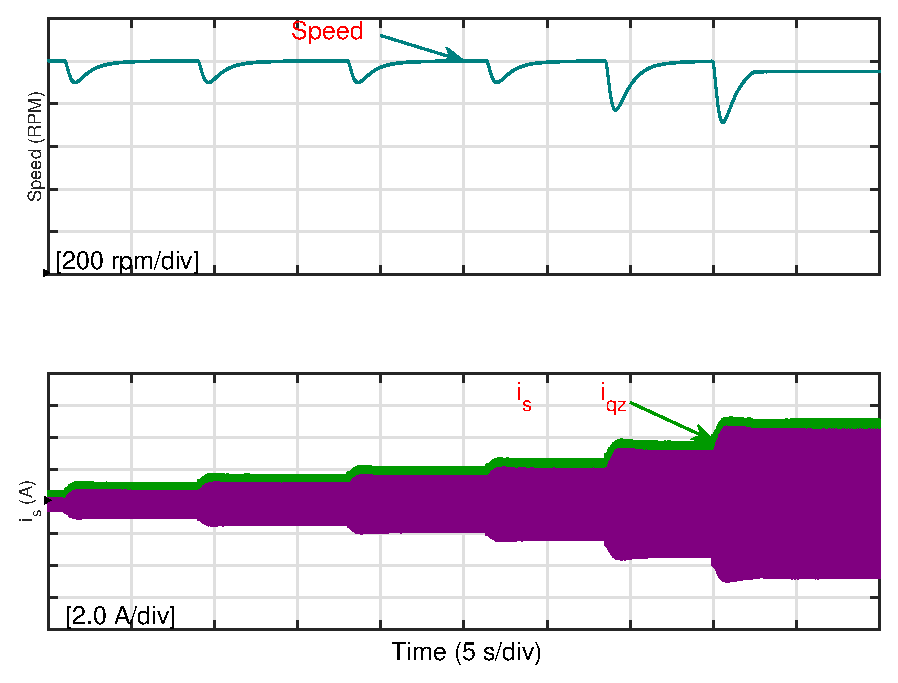
\includegraphics[width=0.6\linewidth]{./PILoadVariation}
  \caption{PI controller under load variation at 50\% rated speed (1000 rpm) with inverter non-linearities
  (dead time, device drops). The composite plot shows motor speed, \(i_q\), and phase currents during torque steps
  from 10\% to 100\% of rated in 20\% increments.}
  \label{fig:PINL_LoadVariation}
\end{figure}

\subsection{Finite Control Set Model Predictive Simulation Modeling Under Inverter-Nonlinearities Effects}
\subsubsection{Steady State Operation}
With dead time and device drops enabled, the FCS–MPC at 1000 rpm and 50\% rated load (\(1.75~\mathrm{N\,m}\)) yields a phase–current THD of 17\% (see Fig.~\ref{fig:FCSNL_1000rpm_med}). The elevated distortion is consistent with single–vector actuation interacting with polarity–dependent voltage biases to project strong odd harmonics—especially \(5^\text{th}\) and \(7^\text{th}\). At this operating point the THD is slightly higher than the PI baseline reported at the same speed (\(\approx\)16.4\%; see Fig.~\ref{fig:PINL_1000rpm_low}).

\begin{figure}[H]
  \centering
  % Replace with your exported plot/image
  
\includegraphics[width=0.6\linewidth]{FCSMidSpeedMidLoadSteadyState}
  \caption{FCS–MPC steady state at 50\% rated speed (1000 rpm) and 50\% rated load (\(1.75~\mathrm{N\,m}\)) with inverter non-linearities (dead time, device drops). The plot shows phase currents, \(d\)- and \(q\)-axis currents, and THD.}
  \label{fig:FCSNL_1000rpm_med}
\end{figure}

\subsubsection{Low Speed Operation}
With dead time and device drops enabled, the FCS–MPC struggles at the most challenging operating point: in sensorless mode at 5\% rated speed (100~rpm) and low load, the controller cannot stabilize because the weak back-EMF and single-vector actuation make the effective voltage quantization too coarse for reliable angle/torque regulation. From 10\% rated (200~rpm) upward the loop settles; at low load the harmonic content remains high—THD 34\%, as shown in Fig.~\ref{fig:FCSNL_200rpm_low}—whereas at high load the larger commanded voltage reduces the vector mismatch and THD drops to 5.6\%, see Fig.~\ref{fig:FCSNL_200rpm_high}. Compared to PI at the same conditions (23\% at low load, 6.9\% at high load), FCS is inferior at light load but shows an advantage at high torque.
% Requires in preamble:
% \usepackage{graphicx}
% \usepackage{subcaption}

\begin{figure}[H]
  \centering
  % --- (a) Low load @ 10% speed (200 rpm) ---
  \begin{subfigure}{0.485\textwidth}
    \centering
    % Replace with your exported plot/image
    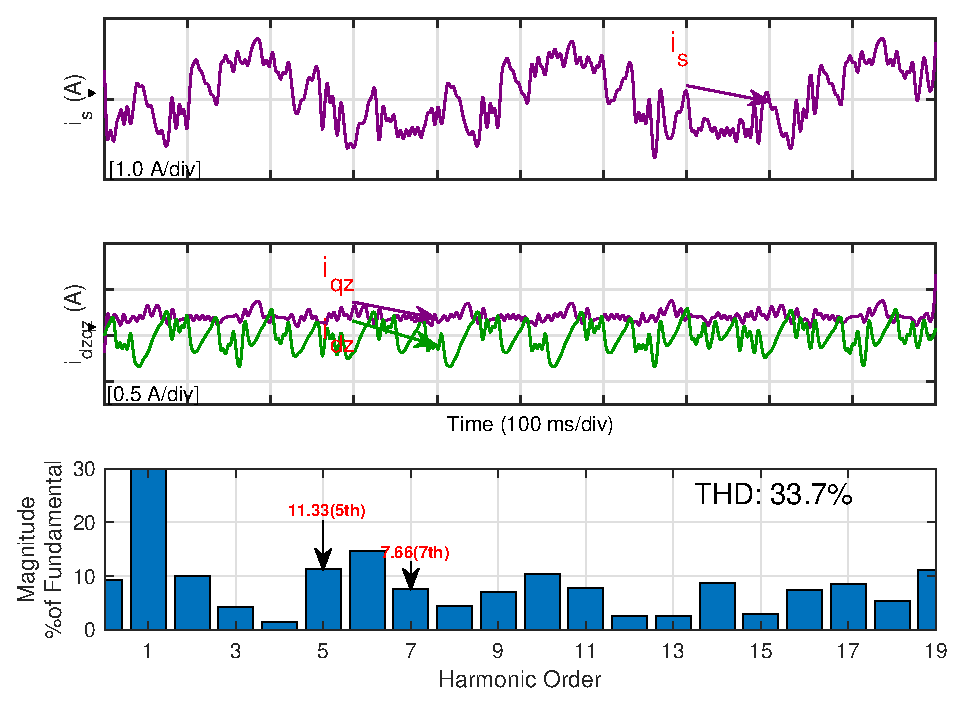
\includegraphics[width=\linewidth]{FCSSteadyStateLowLoad200Rpm}
    \caption{Low load: \(T=0.3~\mathrm{N\,m}\). THD \(=34\%\).}
    \label{fig:FCSNL_200rpm_low}
  \end{subfigure}\hfill
  % --- (b) High/rated load @ 10% speed (200 rpm) ---
  \begin{subfigure}{0.485\textwidth}
    \centering
    % Replace with your exported plot/image
    
\includegraphics[width=\linewidth]{FCSSteadyStateHighLoad200Rpm}
    \caption{Rated load: \(T=3.5~\mathrm{N\,m}\). THD \(=5.6\%\).}
    \label{fig:FCSNL_200rpm_high}
  \end{subfigure}

  \caption{FCS–MPC at 10\% rated speed (200 rpm) with inverter non-linearities (dead time, device drops). 
  Each panel shows phase currents, \(i_{dq}\), and THD.}
  \label{fig:FCSNL_200rpm}
\end{figure}

\subsubsection{Dynamic Performance}
With dead time and device drops enabled, the FCS–MPC was commanded over 5–50\% rated (100–1000~rpm) at \emph{low load} (\(0.3~\mathrm{N\,m}\)). As shown in Fig.~\ref{fig:FCSNL_Dyn_low}, tracking at higher set-points is acceptable, but the step-down to 10\% (200~rpm) loses stability: weak back-EMF and additive voltage bias degrade the sensorless angle SNR, bias one-step predictions, and—under single-vector actuation—lead to suboptimal vector choices and coarse staircase voltages; the loop oscillates and fails to settle, evidencing degraded dynamic robustness in this regime.
% Requires in preamble:
% \usepackage{graphicx}

\begin{figure}[H]
  \centering
  % Replace with your exported plot/image for the low-load dynamic test
  
\includegraphics[width=0.6\linewidth]{./FCSDynamicResponseLowLoad}
  \caption{FCS–MPC dynamic performance under inverter non-linearities at low load (\(T=0.3~\mathrm{N\,m}\)).
  The figure aggregates multiple speed transitions within the 5–50\% rated band (100–1000 rpm), showing command vs.\ speed,
  \(d\)- and \(q\)-axis currents, and phase currents.}
  \label{fig:FCSNL_Dyn_low}
\end{figure}

\subsubsection{Parameter Variation}
At 10\% rated speed (200~rpm) with dead time and device drops enabled, the FCS–MPC was run using a deliberately biased prediction model (\(R_s{+}25\%\), \(L_{d,q}{-}25\%\)) while the plant remained unchanged. As illustrated in Fig.~\ref{fig:FCSNL_ParamVariation}, under the low-load case (\(T\!\approx\!0.3~\mathrm{N\,m}\)) the phase-current THD increases from 34\% (nominal model) to 40\%. This is characteristic of FCS: one-step predictions pick a single vector each sample, so \(R\!-\!L\) errors misrank candidates and, in the presence of polarity-dependent inverter biases, exacerbate the staircase voltage, amplifying harmonics and torque ripple.
% Requires in preamble:
% \usepackage{graphicx}

\begin{figure}[H]
  \centering
  % Replace with your exported composite plot (e.g., speed, dq currents, phase currents, THD bars)
  
\includegraphics[width=0.6\linewidth]{FCSParameterVariation}
  \caption{FCS–MPC with inverter non-linearities (dead time, device drops) under parameter variation at 10\% rated speed (200 rpm, low load \(T\!\approx\!0.3~\mathrm{N\,m}\)).
  The prediction model is biased with \(R_s{+}25\%\) and \(L_{d,q}{-}25\%\) while the plant is unchanged. The composite plot shows \(d\)- and \(q\)-axis currents, phase currents, and THD.}
  \label{fig:FCSNL_ParamVariation}
\end{figure}

\subsubsection{Load Variation}
With dead time and device drops enabled, the motor was held at 1000 rpm while the load torque stepped from 10\% to 100\% of rated in 20\% increments. As shown in Fig.~\ref{fig:FCSNL_LoadVariation}, the FCS–MPC maintains the commanded speed without failures or steady-state deviation—\(i_q\) rises in proportional steps and the average torque matches the request—yet the phase currents exhibit pronounced ripple and the electromagnetic torque shows a high ripple floor. This follows from FCS’s single-vector actuation, whose staircase phase voltage, compounded by polarity-dependent inverter biases, injects strong low-order harmonics despite robust regulation during the load sweep.
% Requires in preamble:
% \usepackage{graphicx}

\begin{figure}[H]
  \centering
  % Replace with your exported composite plot (speed, i_q, phase currents, torque ripple if available)
  
\includegraphics[width=0.6\linewidth]{FCSLoadVariation}
  \caption{FCS–MPC under load variation at 50\% rated speed (1000 rpm) with inverter non-linearities
  (dead time, device drops). The composite plot shows motorspeed, \(i_q\), and phase currents during torque steps
  from 10\% to 100\% of rated in 20\% increments.}
  \label{fig:FCSNL_LoadVariation}
\end{figure}

\subsection{Modulated Model Predictive Controller Simulation Modeling Under Inverter-Nonlinearities Effects}
\subsubsection{Steady State Operation}
With dead time and device drops enabled at 1000 rpm, the M2PC sustains tight regulation and markedly lower distortion than PI or FCS across loads. At \emph{low load} (10\% rated torque, \(0.3~\mathrm{N\,m}\)) the phase-current THD is 8\% (vs.\ \(\sim\)16\% for PI), see Fig.~\ref{fig:M2PCNL_1000rpm_low}; at medium load (50\% rated torque, \(1.75~\mathrm{N\,m}\)) it falls to 2\% (vs.\ \(\sim\)4\% for PI and \(\sim\)17\% for FCS), see Fig.~\ref{fig:M2PCNL_1000rpm_med}. The advantage stems from optimizing a continuous average voltage each sample and realizing it via fixed-frequency SVM, which concentrates spectral energy at the carrier and treats non-idealities as additive biases that can be explicitly compensated—thereby suppressing the staircase ripple that penalizes FCS and outperforming the moderate-bandwidth PI loop at the same operating point.

\begin{figure}[H]
  \centering
  % --- (a) Low load (10% rated torque) ---
  \begin{subfigure}{0.485\textwidth}
    \centering
    % Replace with your exported plot/image
    
\includegraphics[width=\linewidth]{MPCMidSpeedLowLoadSteadyState}
    \caption{Low load: \(T=0.3~\mathrm{N\,m}\). \\THD \(=8\%\).}
    \label{fig:M2PCNL_1000rpm_low}
  \end{subfigure}\hfill
  % --- (b) Medium load (50% rated torque) ---
  \begin{subfigure}{0.485\textwidth}
    \centering
    % Replace with your exported plot/image
    
\includegraphics[width=\linewidth]{MPCMidSpeedMidLoadSteadyState}
    \caption{Medium load: \(T=1.75~\mathrm{N\,m}\).\\ THD \(=2\%\).}
    \label{fig:M2PCNL_1000rpm_med}
  \end{subfigure}

  \caption{M2PC steady state at 50\% rated speed (1000 rpm) with inverter non-linearities (dead time, device drops). Each panel shows \(i_{dq}\), phase currents, and THD at both load levels.}
  \label{fig:M2PCNL_1000rpm}
\end{figure}

\newpage
\subsubsection{Low Speed Operation}
With dead time and device drops enabled, the M2PC remains robust in sensorless operation at very low speeds. At 5\% rated (100~rpm), the phase-current THD is 6.9\% at low load (\(0.3~\mathrm{N\,m}\), see Fig.~\ref{fig:M2PCNL_100rpm_low}) and 1.1\% at rated load (\(3.5~\mathrm{N\,m}\), see Fig.~\ref{fig:M2PCNL_100rpm_high}); at this speed both PI and FCS are unstable. At 10\% rated (200~rpm), MPC yields 6.6\% THD at low load (\(0.5~\mathrm{N\,m}\), see Fig.~\ref{fig:M2PCNL_200rpm_low}) and 1.1\% at rated load (\(3.5~\mathrm{N\,m}\), see Fig.~\ref{fig:M2PCNL_200rpm_high}), compared to \(\sim\)34\%/5.6\% for FCS and \(\sim\)23\%/6.9\% for PI.
% Requires in preamble:
% \usepackage{graphicx}
% \usepackage{subcaption}

\begin{figure}[H]
  \centering

  % --- (a) 5% rated (100 rpm), low load ---
  \begin{subfigure}{0.485\textwidth}
    \centering
    
\includegraphics[width=\linewidth]{./MPCSteadyStateLowLoad100Rpm}
    \caption{5\% speed (100 rpm), low load \(T=0.3~\mathrm{N\,m}\); THD \(=6.9\%\).}
    \label{fig:M2PCNL_100rpm_low}
  \end{subfigure}\hfill
  % --- (b) 5% rated (100 rpm), rated load ---
  \begin{subfigure}{0.485\textwidth}
    \centering
    
\includegraphics[width=\linewidth]{./MPCSteadyStateHighLoad100Rpm}
    \caption{5\% speed (100 rpm), rated load \(T=3.5~\mathrm{N\,m}\); THD \(=1.1\%\).}
    \label{fig:M2PCNL_100rpm_high}
  \end{subfigure}

  \vspace{0.6em}

  % --- (c) 10% rated (200 rpm), low load ---
  \begin{subfigure}{0.485\textwidth}
    \centering
    
\includegraphics[width=\linewidth]{./MPCSteadyStateLowLoad200Rpm}
    \caption{10\% speed (200 rpm), low load \(T=0.5~\mathrm{N\,m}\); THD \(=6.6\%\).}
    \label{fig:M2PCNL_200rpm_low}
  \end{subfigure}\hfill
  % --- (d) 10% rated (200 rpm), rated load ---
  \begin{subfigure}{0.485\textwidth}
    \centering
    
\includegraphics[width=\linewidth]{./MPCSteadyStateHighLoad200Rpm}
    \caption{10\% speed (200 rpm), rated load \(T=3.5~\mathrm{N\,m}\); THD \(=1.1\%\).}
    \label{fig:M2PCNL_200rpm_high}
  \end{subfigure}

  \caption{M2PC at low speeds with inverter non-linearities (dead time, device drops). Each panel shows motor speed, \(i_q\), and phase currents. MPC remains stable at 5\% and 10\% of rated speed and achieves low THD across loads.}
  \label{fig:M2PCNL_low_speed}
\end{figure}

\subsubsection{Dynamic Performance}
With dead time and device drops enabled, the M2PC tracks speed commands within the 10–50\% band (100–1000~rpm) cleanly at both low load (\(0.3~\mathrm{N\,m}\); see Fig.~\ref{fig:M2PCNL_Dyn_100to1000_low}) and rated load (\(3.5~\mathrm{N\,m}\); see Fig.~\ref{fig:M2PCNL_Dyn_100to1000_rated}). In all transitions the measured speed follows the reference with overshoot \(\mathbf{<10\%}\) and negligible steady-state error, while \(i_q\) steps proportionally to torque demand. Thanks to optimizing a continuous average voltage each sample and realizing it at fixed switching frequency, the phase currents remain smooth and torque ripple is far lower than FCS and distinctly lower than PI throughout acceleration and deceleration.
% Requires in preamble:
% \usepackage{graphicx}
% \usepackage{subcaption}

\begin{figure}[H]
  \centering
  % --- (a) Low load ---
  \begin{subfigure}{0.485\textwidth}
    \centering
    % Replace with your exported plot/image
    
\includegraphics[width=\linewidth]{MPCDynamicResponseLowLoad}
    \caption{Low load: \(T=0.3~\mathrm{N\,m}\). Overshoot \(<10\%\); smooth \(i_q\)/phase currents.}
    \label{fig:M2PCNL_Dyn_100to1000_low}
  \end{subfigure}\hfill
  % --- (b) Rated load ---
  \begin{subfigure}{0.485\textwidth}
    \centering
    % Replace with your exported plot/image
    
\includegraphics[width=\linewidth]{MPCDynamicResponseHighLoad}
    \caption{Rated load: \(T=3.5~\mathrm{N\,m}\). Overshoot \(<10\%\); very low torque ripple.}
    \label{fig:M2PCNL_Dyn_100to1000_rated}
  \end{subfigure}

  \caption{M2PC dynamic response with inverter non-linearities (dead time, device drops) for speed changes within the \(10\%\!\to\!50\%\) rated band (100–1000 rpm). Each panel shows command vs.\ speed, \(i_q\), and phase currents.}
  \label{fig:M2PCNL_Dyn_100to1000}
\end{figure}

\subsubsection{Parameter Variation}
At 5\% rated speed (100~rpm) with dead time and device drops enabled, the M2PC was run using a biased prediction model (\(R_s{+}25\%\), \(L_{d,q}{-}25\%\)). As shown in Fig.~\ref{fig:M2PCNL_ParamVariation}, the phase-current THD remains 8\%, markedly lower than the PI and FCS results under the same bias (Fig.~\ref{fig:PINL_ParamVariation}: \(\sim\)24\%; Fig.~\ref{fig:FCSNL_ParamVariation}: \(\sim\)40\%). The fixed-frequency SVM realization of an optimized continuous average voltage makes MPC largely insensitive to moderate \(R\!-\!L\) errors and limits the impact of additive inverter distortions, yielding robust low-speed performance.
% Requires in preamble:
% \usepackage{graphicx}

\begin{figure}[H]
  \centering
  % Replace with your exported composite plot (e.g., speed, dq currents, phase currents, THD bar)
  
\includegraphics[width=0.6\linewidth]{MPCParameterVariation}
  \caption{M2PC under parameter variation with inverter non-linearities (dead time, device drops) at
  5\% rated speed (100 rpm). The prediction model is biased with \(R_s{+}25\%\) and \(L_{d,q}{-}25\%\).
  The composite plot shows \(d\)- and \(q\)-axis currents, phase currents, and THD.}
  \label{fig:M2PCNL_ParamVariation}
\end{figure}

\subsubsection{Load Variation}
With dead time and device drops enabled, the motor was held at 1000 rpm while the load torque was stepped from 10\% to 100\% of rated in 20\% increments. As shown in Fig.~\ref{fig:M2PCNL_LoadVariation}, the M2PC maintains the commanded speed without droop, while \(i_q\) increases in clean, proportional steps to furnish the added torque and the phase currents remain smooth thanks to the fixed-frequency SVM realization of the optimized average voltage. The short, well-damped transients visible in Fig.~\ref{fig:M2PCNL_LoadVariation} evidence robust disturbance rejection and low ripple despite inverter non-linearities.
% Requires in preamble:
% \usepackage{graphicx}

\begin{figure}[H]
  \centering
  % Replace with your exported composite plot:
  % (left) speed response, (middle) q-axis current, (right) phase currents
  
\includegraphics[width=0.6\linewidth]{MPCLoadVariation}
  \caption{M2PC under load variation at 50\% rated speed (1000 rpm) with inverter non-linearities
  (dead time, device drops). The composite figure shows command vs.\ speed, \(i_q\), and phase currents during torque steps
  from 10\% to 100\% of rated in 20\% increments.}
  \label{fig:M2PCNL_LoadVariation}
\end{figure}


